\section{Zpětná západka}
\begin{figure}
    \centering
    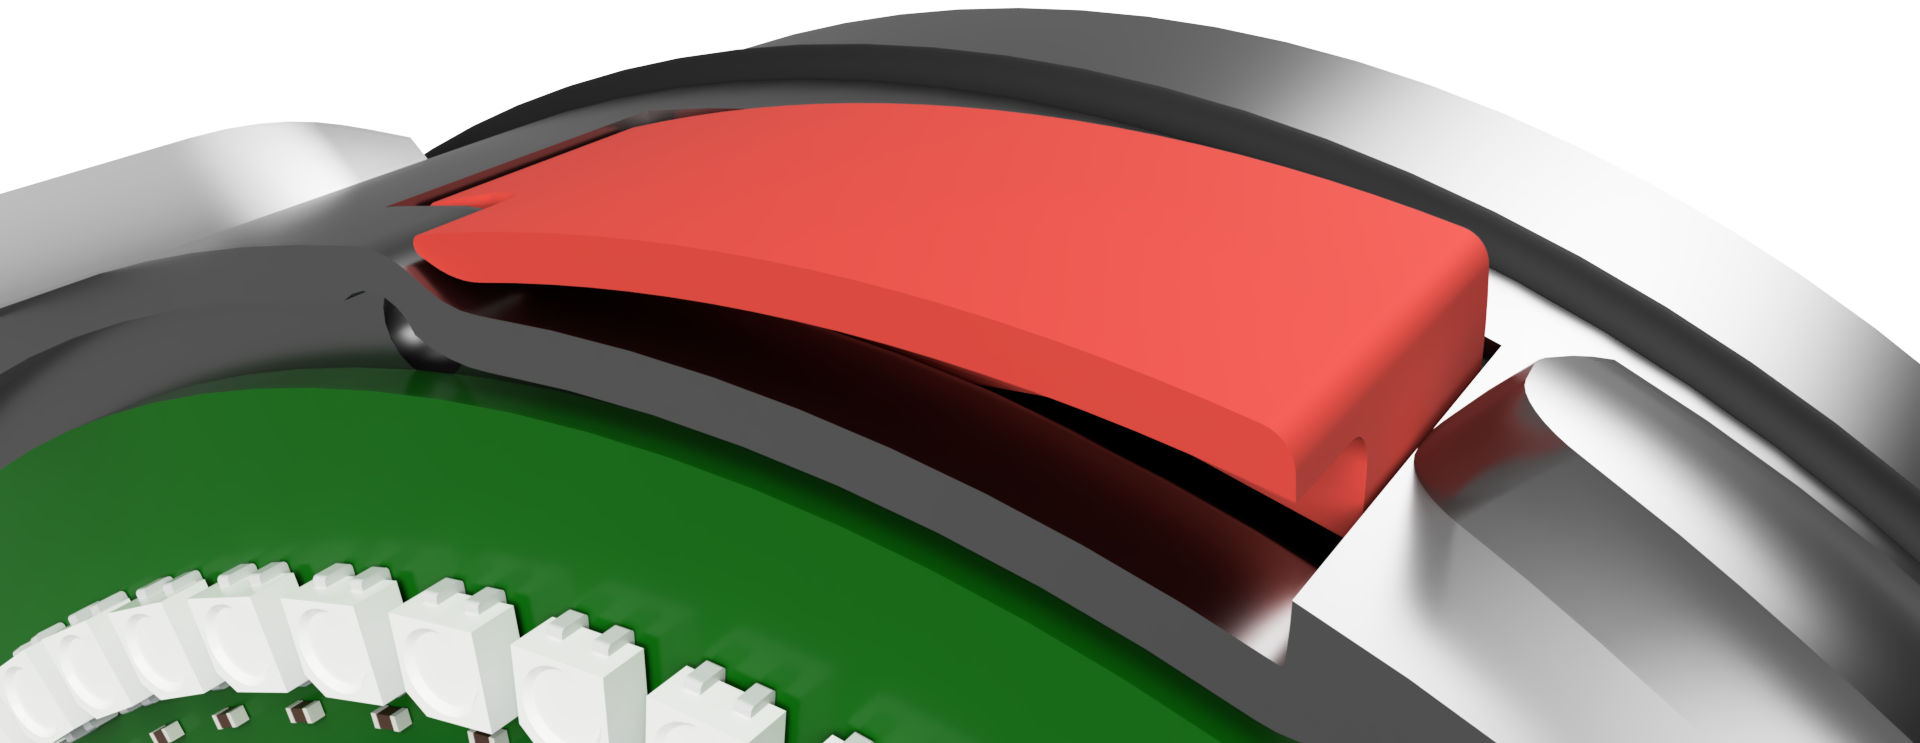
\includegraphics[width=\textwidth]{kapitoly/obrazky/E4/zapadka/render.png}
    \caption{render západky}
    Zpětnou západkou pohybuje motor pomocí magnetu. Pro zajištění voděodolnosti je motor od západky oddělen stěnou, což je také jeden z důvodů 
    použití magnetického spojení.
    \label{fig:E4-zapadka}
\end{figure}

\clearpage
\newpage

\paragraph{Sklon čela}
\addcontentsline{toc}{paragraph}{Sklon čela}

Aby při zamčení západka doléhala na otvor trezoru, a zároveň neměla příliš velkou vůli, je potřebné správně navrhnout tvar západky.
Jednou z možností je navrhnout čelní plochu jako část válcové plochy. Tato plochu také musí být zároveň v otvoru pro dveře.
Sice teoreticky není problém jí na FDM tiskárně vytisknout, pro západku, a na laseru vypálit v otvoru, ale výsledná plocha je hlavně u tisku 
nevzhledná a je třeba jí obrousit do požadovaného vzhledu. Obrousit válcovou plochu je však náročnější než plochu rovnou, zvlášť v otvoru trezoru, 
a je tedy pro mě výhodnější navrhnout tuto plochu jako rovinu a jen jí správně sklonit. Špatně navržený sklon by se projevil buď přílišnou vůlí 
což by znamenalo, že by se dveře v trezoru viklaly a nebo by západka nebyla samosvorná což by se projevilo možností trezor otevřít vetší silou 
i bez jeho odemčení.

\begin{figure}[htbp]
    \centering
    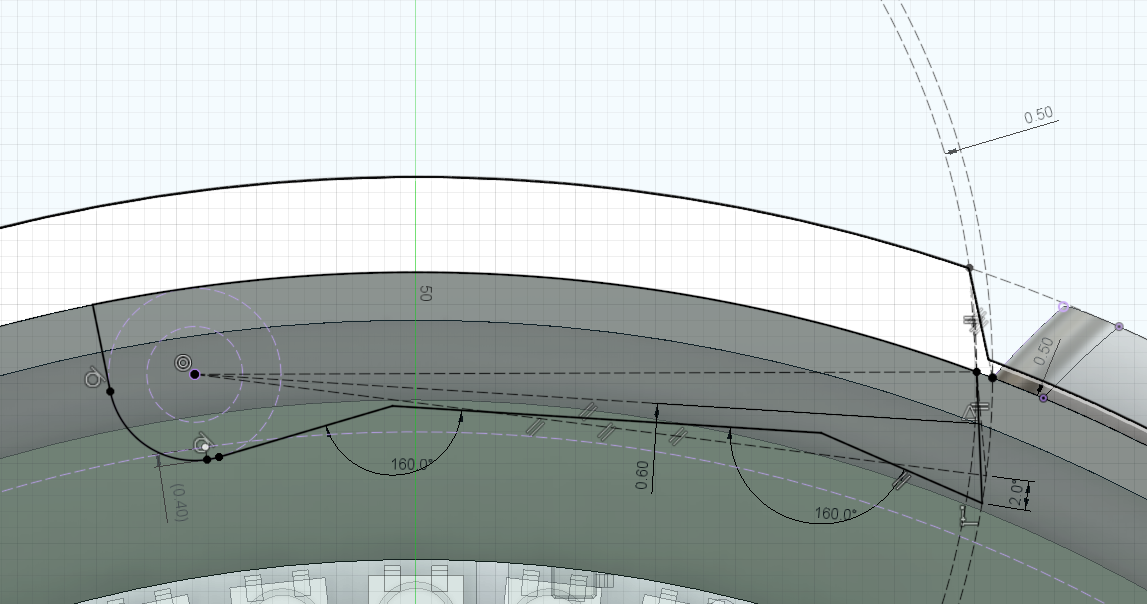
\includegraphics[width=\textwidth]{kapitoly/obrazky/E4/zapadka/uhel_cela.png}
    \caption{}
    \label{fig:E4-uhel_cela_zapadky}
\end{figure}

\newpage
\paragraph{západka v průběhu vývoje}
\addcontentsline{toc}{paragraph}{západka v průběhu vývoje}

Západka se ve vývoji pochopitelně objevila společně s bajonetem ale v první verzi byla jen částí těla dveří a teprve v dalších verzích se stala
samostatnou součástkou. První tělo využívající bajonet jsem tiskl na FDM tiskárně z plastu PLA a západka byla jen jeho pružnou částí. Toto řešení sice 
z počátku fungovalo a mělo výhodu jednoduší výroby, ale PLA po několika měsících začalo ztrácet pružnost a západka se už nepohybovala v celém rozsahu.
Toto jsem z počátku chtěl řešit samostatnou západkou ve spojení s tažnou pružinou. Pružina však nebyla třeba a naprosto stačí magnet na motoru a v západce.
Západka proto zůstala v teto podobě a jen se přidala mechanická přepážka kvůli voděodolnosti. 

\begin{figure}[htbp]
    \paragraph{simulace odolnosti proti násilnému vniknutí}
    \addcontentsline{toc}{paragraph}{simulace odolnosti proti násilnému vniknutí}
    Vzhledem k tomu že západka je součást která při zamčení brání otevření je třeba aby odolala při pokusech dveře otevřít bez odemčení.
    \centering
    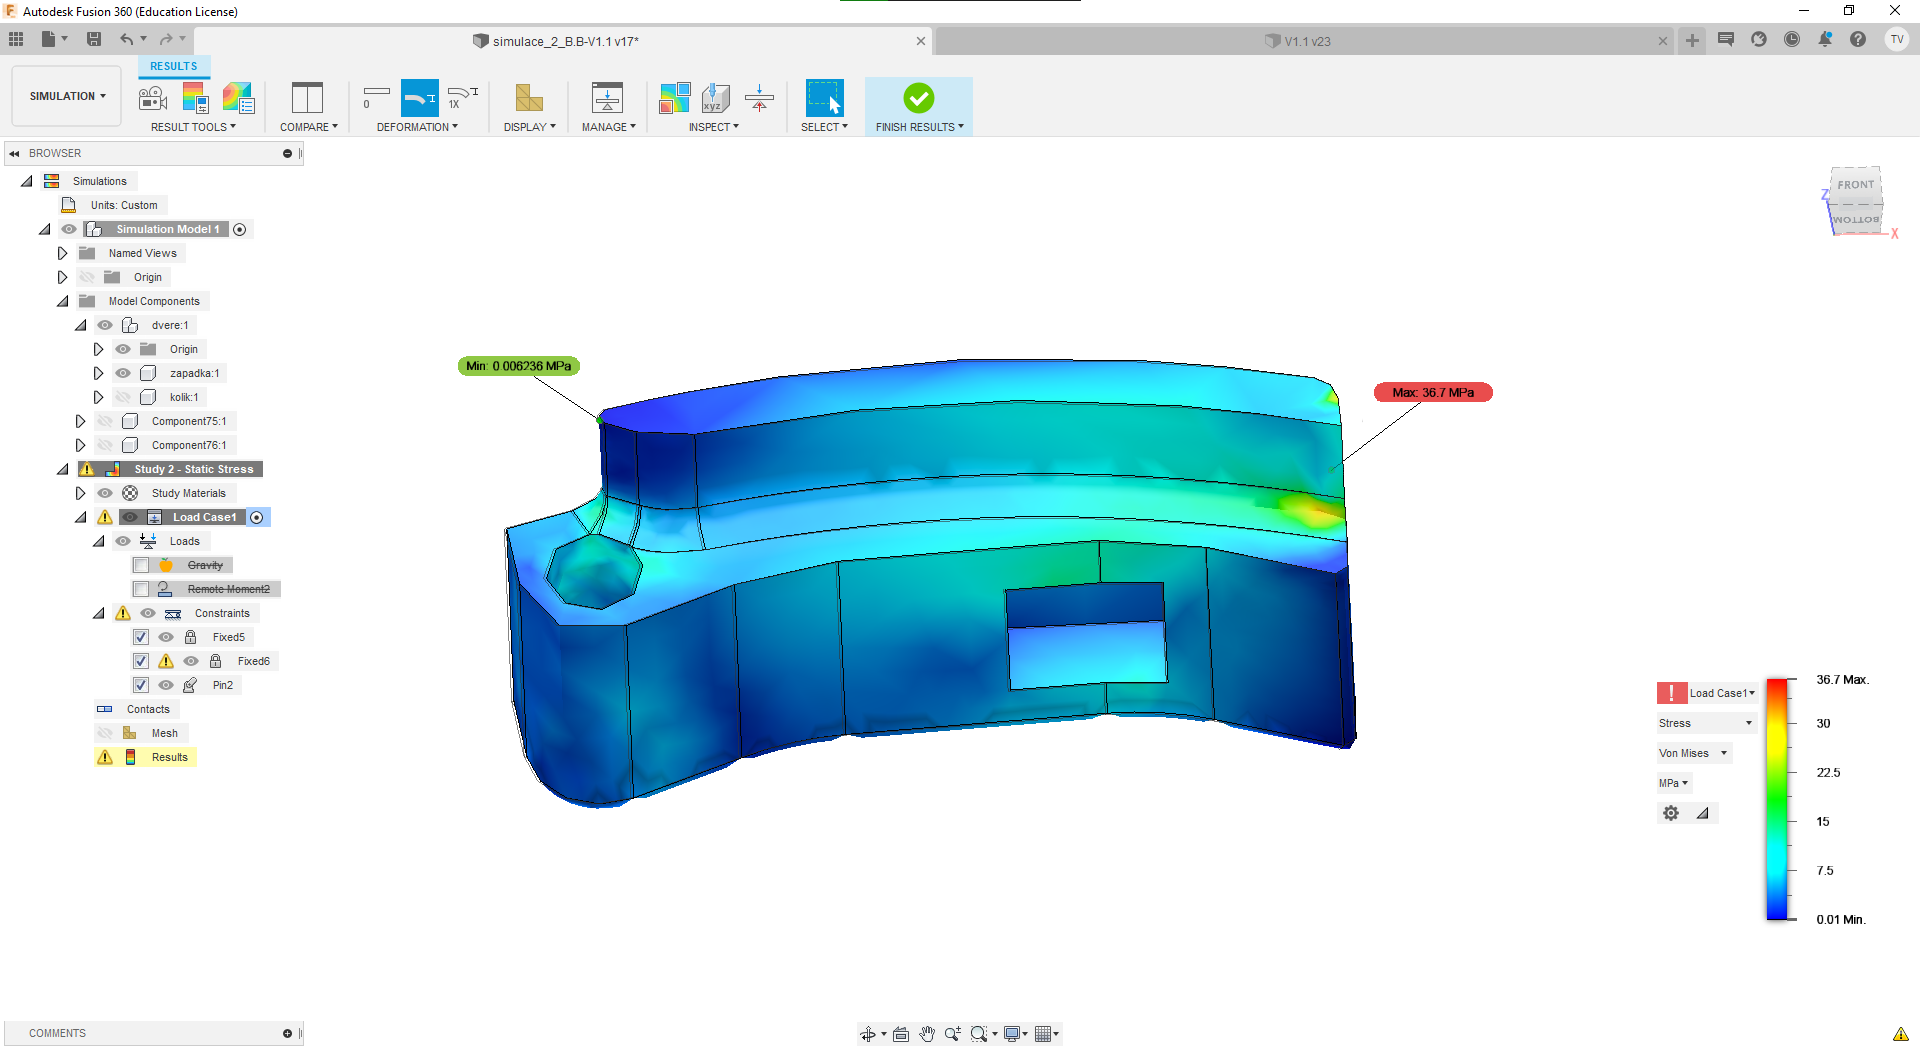
\includegraphics[width=\textwidth]{kapitoly/obrazky/E4/zapadka/simulace/napeti_D1-M5000.png}
    \caption{simulace napětí v západce při kroutícím momentu 5000 N*mm což na rameni 48mm znamená sílu působící na kolík 104N}
    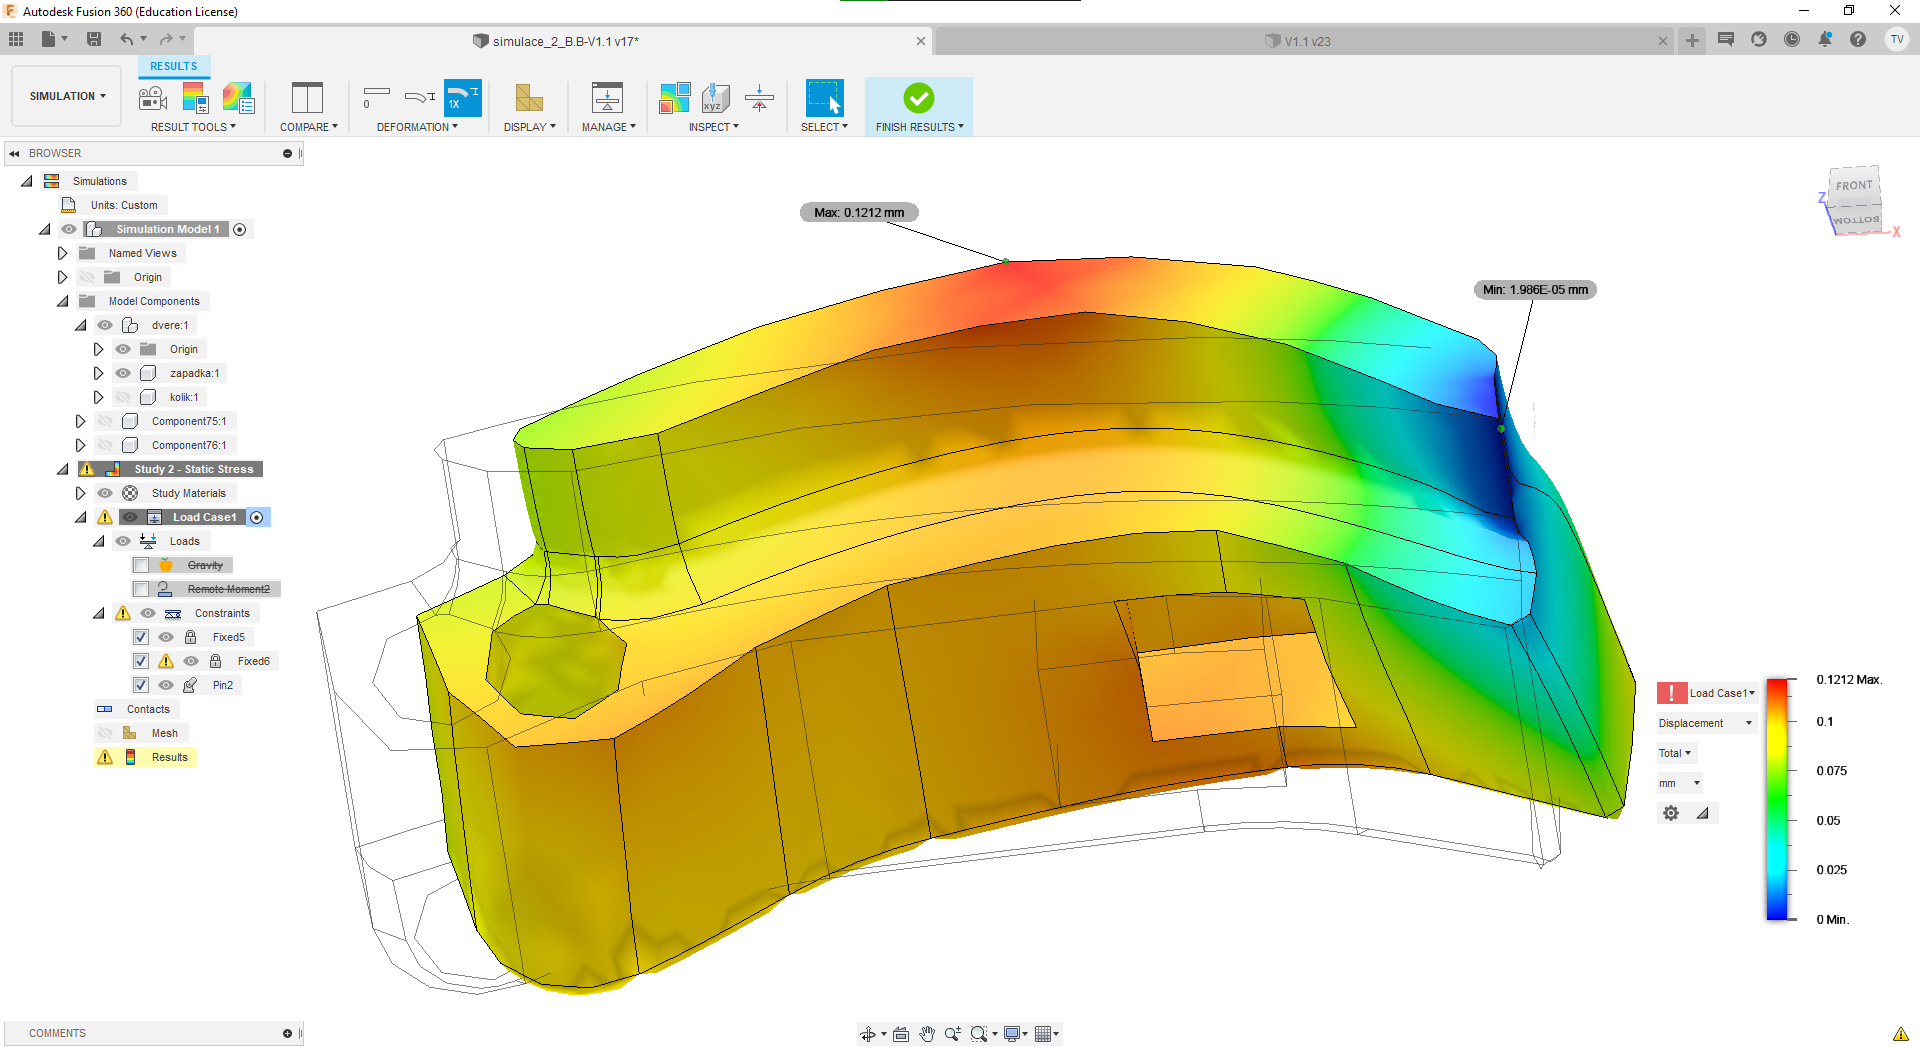
\includegraphics[width=\textwidth]{kapitoly/obrazky/E4/zapadka/simulace/Dislokace_D10-M5000.png}
    \caption{zobrazení deformace, pro lepší zobrazení je deformace zdesetinásobená}
    \label{fig:E4-simulace_zapadky}
\end{figure}

%    Západka
%        / a) vývoj západky
%        /     1) původní verze (pružnost materiálu -> po čase ztrácí pružnost)
%        /     2) verze s pružinou (pružina je nepotřebná a jsou s ní zbytečné problémy)
%        /     3) b,c,d,e
%        b) obrázek
%        // c) uhel čela (tak aby měla dosedací plocha co nejmenší vůli a zároveň opravdu dosedala v celé ploše [a ne v úseče nebo dokonce jednom bodě])
%        //    1) obrázek
%        d) pohyby
%            1) pohyb tam
%            2) pohyb spět (stačí magnet pružina je nepotřebná)
%            3) motor
%            4) enkoder
%            5) možná video?
%        e) matika
%        //    1) odolnost proti zpětnému otočení
%        //    2) obrázek ze simulace
%        --    3) možná video?

\newpage